\section*{Ziel}
Im folgenden Versuch soll die Eigenschaften eines Lasers untersucht werden. 
Dazu wird unteranderem die Wellenlänge, die Polarisation, das Modenspektrum und die Intensitätsverteilung in der Ebene senkrecht zur Ausbreitungsrichtung betrachtet.
Geprüft wird Stabilitätsbedingung des Resonators, 2 TEM-Moden des Lasers, sowie die Beugung an einem Strichgitter.
\section{Theorie}
\subsection{Funktionsweise eines Lasers}
Ein Laser (Light Amplification by Stimulated Emission of Radiation) besteht grundsätzlich aus drei verschiedenen
Komponenten. Diese befassen das Lasermedium, ein Resonator und eine Pumpquelle. Das Lasermedium bestimmt dabei durch optische Übergänge
das Strahlenspektrum des Lasers, sodass dieser monochromatisches Licht hoher Intensität und Kohärenz erreicht.
Der Resonator bildet die Grundlage für eine selbstanregende Oszillation, sodass eine optische Rückkopplung des ausgestrahlten Laser entsteht und somit wiederholt
durch das Lasermedium geleitet wird. Energie wird dem System über die Pumpquelle hinzugefügt, sodass es zur einer Inversion kommt.
Umfassend lässt sich sagen, dass das Strahlungsfeld in jener Art und Wiese mit dem Lasermedium wechselwirkt, sodass das einfallende Licht verstärkt wird.
\subsection{Zwei-Niveau-System}
Zunächst wird das Zwei-Niveau-System betrachtet. Auch wenn sich dieses für den Laser nicht nutzen lässt, soll zunächst zum
Verständnis der Zustandssysteme beitragen.\\
Bei dem Helium-Neon-Laser handelt es sich um enen Gasentaldungslaser. Das enthaltende Medium hat dabei
zwei mögliche Energiezustände $E_1$ und $E_2$ in denen sich jeweils $N_1$ und $N_2$ Teilchen befinden (Besetzungszahl).
Durch die Pumpquelle können die Teilchen nun auf das höhere Energieniveau $E_2$ angeregt werden.
Folgende drei Prozesse, dargestellt in Abbildung \ref{fig:3wege} können dabei auftreten.
\subsubsection*{Anregung durch Absorbtion}
Dabei bringt ein Photon, welches mindestend die Energie $\Delta E=E_2-E_1$ besitzt, das Teilchen vom Grundzustand in den angeregten Zustand.
\subsubsection*{Spontane Emission}
Das angeregte Atom emittiert spontan ein Photon in beliebige Richtung und kehr somit in den Grundzustand zurück.
\subsubsection*{Induzierte Emission}
Ein Photon mit der Energie zwischen angeregtem Zustand und Grundzustand löst einen Übergang im Medium aus. Das entstehende stimulierte Photon
bewegt sich in die selbe Richtung, bei gleicher Energie, Phasenlage und P0larisation.

\begin{figure}
    \center
    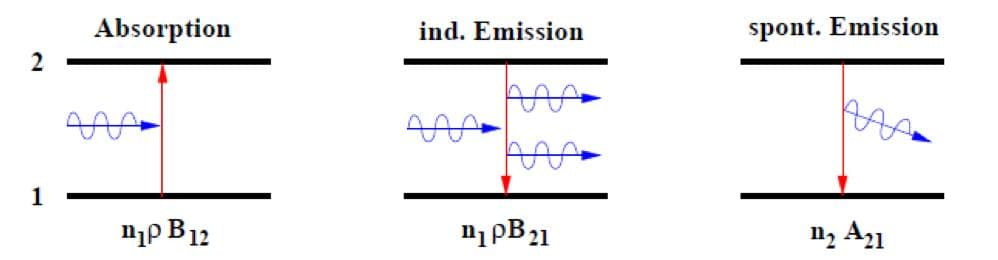
\includegraphics[width=0.8\textwidth]{bilder/3wege.jpg}
    \caption{Absorbtion und Emission schematisch Dargestellt für ein Strahlungsfeld $\rho(\nu)$ in einem Zweizustandssystem \cite{anleitung}}
    \label{fig:3wege}
\end{figure}
\label{sec:theorie}

Für die absorbierten und emittierten Photonen gilt $\omega=\frac{\Delta E}{\hbar}$ und die Different $\Delta N$ bezeichnet man als Inversion.
Durch die Anregung folgt eine zeitliche Änderung der Besetzungszahlen $N_1$ und $N_2$, die sich schreibt lassen als
\begin{align}
    \frac{dN_1}{dt}&=-N_1\rho B_{12}+N_2\rho B_{21} + N_2 A_{21}\\
    \frac{dn_2}{dt}&=+N_1\rho B_{12}-N_2\rho B_{21} - N_2 A_{21}= -\frac{dN_1}{dt}.
\end{align}
Dabei spiegelt $A_{21}$ den Einsteinkoeffizienten für spontane Emission, $B_{12}$ für Absorbtion und $\rho$ die spektrale Strahldickte im Resonator wieder.
Da gilt
\begin{align}
    N&=N_1+N_2{,}\\
    \Delta N &= N_2-N_1{,}\\
    B_{12}&=B_{21}:=B{,}\\
    A_{21}&:=A{,}   
\end{align}
folgt somit
\begin{equation}
    \frac{d\Delta N}{dt}=-2B\rho\Delta N + AN-A\Delta N.
\end{equation}
Da aufgrund des thermischen Gleichgewichtes (Maxwell-Boltzmann-Verteilung) mehr Teilchen den Grundzustand besetzten und somit maximal eine 
Gleichbesetztung der beiden Energiezustände erreicht werden kann, lässt sich ein Laser durch ein Zweizustandssystem nicht realisieren. Kurz gesagt,
es lässt sich keine Inversion (angeregter Zustand iegt öfter vor als Grundzustand) erreichen.
Dies ist allerdings notwendig, damit die stimulierte Emission häufiger als die induzierte Emission auftritt und somit die gewünschte Verstärkung des Strahlungsfeldes auftritt.
Sodass eine permanente Energiezufuhr durch das Pumpen nötig ist.

\subsection{Der Resonator}
Da die gewünschte Verstärkung exponentziell von der Länge des Laufweges im ativen Lasermedium abhängt, ist die Nutzung eines optischen Resonators sinnvoll.
Realsisert wird dieser durch zwei sich gegenüberliegenden totalreflektierenden (geringe Transmission) Spiegeln (dargestellt in Abbildung \ref{fig:resonator}).

\begin{figure}
    \center
    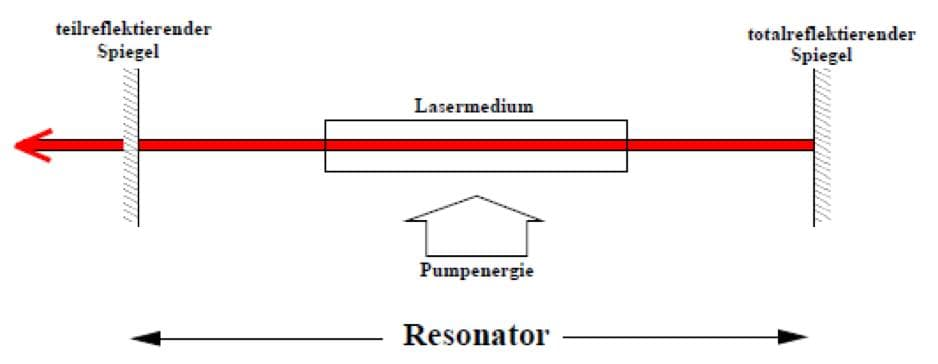
\includegraphics[width=0.8\textwidth]{bilder/resonator.jpg}
    \caption{Schematische Darstellung des Resonators mit zwei totalreflektierenden Speigeln \cite{anleitung}.}
    \label{fig:resonator}
\end{figure}